%% two-column format
%\documentclass[9pt,twocolumn]{jctc}   % to mimic appearance in journal

%% one-column format
%%\documentclass[9pt,onecolumn]{jpc}   % to mimic appearance in journal
%%\renewcommand{\baselinestretch}{2.0}

%% We will be using PDF figures and generating PDF output.
%\pdfoutput=1
%\pdfcompresslevel=9
%\usepackage[pdftex]{graphicx}
%\DeclareGraphicsExtensions{.pdf}

%% The figures are in a figures/ subdirectory.
%\graphicspath{{figures/}}

%% Import useful packages.
%\usepackage{times}                             	   % nice fonts
%\usepackage{amsmath}                           % for 'case'
%\usepackage{amsthm}                             % for theorems and proofs
%\usepackage{mathrsfs}                            % script math font
%\usepackage{url}                                	   % allow use of URLs
%\usepackage{latexsym}                            % some math symbols, like \Box
%\usepackage{subfigure}                           % allow use of subfigures

%% Define some useful commands we will use repeatedly.
%\newcommand{\T}{\mathrm{T}}                                % T used in matrix transpose
%\newcommand{\tauarrow}{\stackrel{\tau}{\rightarrow}}       % the symbol tau over a right arrow
%\newcommand{\expect}[1]{\langle #1 \rangle}                % <.> for denoting expectations over realizations of an experiment or thermal averages
%\newcommand{\estimator}[1]{\hat{#1}}                       % estimator for some quantity from a finite dataset.
%\newcommand{\code}[1]{{\tt #1}}

%%% DOCUMENT %%%%%%%%%%%%%%%%%%%%%%%%%%%%%%%%%%%%%%%%%%%%%%%%%%%%%%%%%%%%%%%%%%%%
%\begin{document}

%% TITLE %%%%%%%%%%%%%%%%%%%%%%%%%%%%%%%%%%%%%%%%%%%%%%%%%%%%%%%%%%%%%%%%%%%%

The material in this chapter was submitted to the Journal of Chemical Theory and Computation, and has been accepted to appear as:

\flushleft{\bf Use of the Weighted Histogram Analysis Method for the Analysis of Simulated and Parallel Tempering Simulations}

\flushleft{{\bf John D. Chodera\thanks{Author to whom correspondence is to be addressed: John D. Chodera {\tt <jchodera@gmail.com>}}$\:\:^\dag$, William C. Swope$^\ddag$, Jed W. Pitera$^\ddag$, Chaok Seok$^\S$, and Ken A. Dill$^\P$} \\
\emph{\normalsize $^\dag$ Graduate Group in Biophysics and $^\P$ Department of Pharmaceutical Chemistry, University of California at San Francisco, San Francisco, CA 94143} \\
\emph{\normalsize $^\ddag$ IBM Almaden Research Center, 650 Harry Road, San Jose, CA 95120} \\
\emph{\normalsize $^\S$ Department of Chemistry, College of Natural Sciences, Seoul National University, Gwanak-gu, Shillim-dong, san 56-1 Seoul 151-747, Republic of Korea}}

%\maketitle
%\date{}

%% ABSTRACT %%%%%%%%%%%%%%%%%%%%%%%%%%%%%%%%%%%%%%%%%%%%%%%%%%%%%%%%%%%%%%%%%%%%
\section*{Abstract}

The growing adoption of generalized-ensemble algorithms \cite{okamoto:2004a} for biomolecular simulation has resulted in a resurgence in the use of the weighted histogram analysis method (WHAM) \cite{kumar:1992a} to make use of all data generated by these simulations.  Unfortunately, the original presentation of WHAM by Kumar \emph{et al.} \cite{kumar:1992a} is not directly applicable to data generated by these methods.  WHAM was originally formulated to combine data from independent samplings of the \emph{canonical} ensemble, whereas many generalized-ensemble algorithms sample from mixtures of canonical ensembles at different temperatures.  Sorting configurations generated from a parallel tempering simulation by temperature obscures the temporal correlation in the data and results in an improper treatment of the statistical uncertainties used in constructing the estimate of the density of states.  Here we present variants of WHAM, derived with the same set of assumptions, that can be directly applied to several generalized ensemble algorithms, including simulated tempering \cite{mitsutake:2000a}, parallel tempering (better known as replica-exchange among temperatures) \cite{sugita:1999a}, and replica-exchange simulated tempering \cite{mitsutake:2000a}.  We present methods that explicitly capture the considerable temporal correlation in sequentially generated configurations using autocorrelation analysis.  This allows estimation of the statistical uncertainty in WHAM estimates of expectations for the canonical ensemble.  We test the method with a one-dimensional model system, and then apply it to the estimation of potentials of mean force from parallel tempering simulations of the alanine dipeptide in both implicit and explicit solvent.

%% INTRODUCTION %%%%%%%%%%%%%%%%%%%%%%%%%%%%%%%%%%%%%%%%%%%%%%%%%%%%%%%%%%%%%%%%
\section{Introduction}

The difficulty of computing equilibrium averages for complex systems such as solvated biopolymers by Monte Carlo or molecular dynamics simulation is well-known.  Numerous minima and large free-energy barriers tend to slow exploration in phase space and trap the simulation in metastable regions of configuration space.  This hampers the ability of the system both to equilibrate (reach the thermodynamically relevant region of phase space) and to sample sufficiently for estimates of ensemble averages to converge (reduce the statistical uncertainty in the estimate to an acceptable level) in finite computer time.

The emergence of a new class of simulation algorithms, termed \emph{generalized-ensemble} algorithms \cite{okamoto:2004a}, has helped to mitigate these problems.  In a generalized-ensemble simulation, the probability distribution from which conformations are sampled is altered from a canonical distribution to one that will induce a broader sampling of the potential energy.  Proper application should in principle allow the system to overcome energetic barriers and sample configuration space more thoroughly, at the expense of spending more time in high-energy regions that may be irrelevant at the temperature of interest.  The particular method by which sampling is enhanced depends on the algorithm. In the \emph{multicanonical algorithm} (MUCA) \cite{berg:1991a,berg:1992a,hansmann:1993a,nakajima:1997a,yasar:2000a}, conformations are sampled with a probability proportional to an approximation of the inverse potential energy density of states in an attempt to produce a random walk in the potential energy.  In \emph{simulated tempering} (ST) \cite{marinari:1992a,lyubartsev:1992a,mitsutake:2000a}, a random walk between canonical ensembles at different temperatures is used to produce a random walk in energy, but an estimate of the free energy as a function of temperature is needed as input to ensure equal visitation of all temperatures.  \emph{Parallel tempering} (PT), a special case of the replica-exchange method (REM) \cite{hansmann:1997a,sugita:1999a}, eliminates the need to know these free energies \emph{a priori} by coupling temperature changes between pairs of a pool of simulated tempering simulations conducted in parallel.  Several other algorithms and combinations thereof have also been proposed \cite{mitsutake:2000a,mitsutake:2003a,mitsutake:2004a,sugita:2000b}.

In several of these algorithms, such as simulated tempering and parallel tempering, each replica generates configurations from a \emph{mixed-canonical} distribution (a term coined in \cite{fischer:1998a}) --- that is, a number of configurations are generated from the canonical distribution at each of several temperatures.  To compute expectations over the canonical ensemble at a single temperature, either the configurations from all replicas that visit the temperature of interest must be collected and the remainder discarded (as in \cite{sanbonmatsu:2002a}) or else a reweighting scheme must be used to properly weight the data generated at other temperatures.  Fortunately, the weighted histogram analysis method (WHAM) \cite{kumar:1992a}, an extension of the single- and multiple-histogram methods introduced by Ferrenberg and Swendsen \cite{ferrenberg:1988a,ferrenberg:1989a}, allows configurations generated from independent canonical simulations at different temperatures to be reweighted to compute expectations from the canonical ensemble at any temperature of interest.  Okamoto and coworkers have applied this method to both replica-exchange simulated tempering (REST) \cite{mitsutake:2000a} and parallel tempering \cite{sugita:1999a} methods by reordering sampled configurations into pseudotrajectories, grouping configurations generated at a particular temperature together regardless of which replica they came from.  Unfortunately, this permutation obscures the correlation among the stored configurations, causing the apparent correlation times for each pseudotrajectory to appear artificially shorter than the true correlation times within the independent replica trajectories.  The permutation also introduces correlation \emph{between} the pseudotrajectories, which is problematic because WHAM as presented in \cite{kumar:1992a} is constructed to operate on \emph{independent} canonical trajectories.  Additionally, it is difficult to estimate the statistical uncertainty in the resulting estimate of the expectation from these pseudotrajectories, since standard autocorrelation analysis techniques \cite{mueller-krumbhaar:1973a,swope:1982a,flyvbjerg:1989a,janke:2002a} can no longer be applied.  Recently, Gallicchio \emph{et al.} \cite{gallicchio:2005a} have described a new method for computing expectations and uncertainties from canonical simulations at different temperatures based on Bayesian inference.  While Bayesian approaches are usually superior to those based on first-order Taylor expansion methods for the propagation of uncertainties (of the sort we describe in this work), they are less suitable for treating highly correlated measurements where the functional form of the correlation is essentially unknown.

Here, we derive variants of WHAM that operate on replica trajectories that are not reordered or collected by temperature.  It should be noted that even if simulation data has been stored to disk sorted by temperature, it can be permuted back to the original replica trajectories to perform the proposed analyses if information about the replica-to-temperature mapping or swapping was stored.  Our presentation takes a careful approach to the correlation times involved, and we show under which conditions the almost universally omitted statistical inefficiency term that appears in all formulations of WHAM-like methods can be properly neglected.  Finally, we show how the statistical uncertainty in the estimator for the configuration space average for some observable can be estimated by considering the effect of temporal correlation.  The method is simple and inexpensive enough to employ in all cases where WHAM is used, and we hope all researchers using WHAM will report these statistical uncertainties in future to assess both the significance and the degree of reproducibility of results from simulations.

This paper is organized as follows: In Section \ref{wham:section:wham-review}, we present a derivation of the Kumar \emph{et al.} WHAM for independent simulations sampling from the canonical ensemble.  Careful attention is paid to the proper treatment of time correlation in estimating the statistical uncertainty in the histograms and the resulting estimator for the expectation, and a novel way of obtaining estimates for multiple observables is presented.  In Section \ref{wham:section:simulated-and-parallel-tempering}, we derive an analogue of the method for treating simulated and parallel tempering simulations while properly capturing the correlations among sequential configurations. In Section \ref{wham:section:applications}, we validate our uncertainty estimates in a one-dimensional model system and demonstrate an application for biomolecular systems by estimating the potential of mean force and corresponding uncertainties from parallel tempering simulations of alanine dipeptide in implicit and explicit solvent.  An illustrative efficient implementation of the method in Fortran 95 for use in the analysis of simulated and parallel tempering simulations can be found in the Supplementary Material, and a version that can be compiled and run can be downloaded online\footnote{An implementation of the method for the analysis of simulated parallel tempering simulations can be found at \url{http://www.dillgroup.ucsf.edu/~jchodera/code/wham}.}.

%% REVIEW OF WHAM FOR CANONICAL SIMULATIONS %%%%%%%%%%%%%%%%%%%%%%%%%%%%%%%%%%%%%%%%%%%%%%%%
\section{Independent Canonical Simulations}
\label{wham:section:wham-review}

In this section, we review the derivation of WHAM for computing expectations from multiple independent simulations in the canonical ensemble.  Conducting independent simulations at the same or different temperatures can reduce statistical uncertainty while obtaining perfect parallelism (after the initial time to reach equilibrium has been discarded).  Some of these simulations might be conducted at a higher temperature than the temperature of interest to promote greater sampling across barriers, for example.  Sometimes, the expectation value of one or more observables is desired over a range of temperatures.  Additionally, simulations started from different initial conditions can be used as a check of equilibration and convergence \cite{gelman:1992a}. Below, we follow roughly the same approach as Kumar \emph{et al.} \cite{kumar:1992a} in deriving the WHAM equations, though our notation differs substantially and we include a more detailed treatment of statistical uncertainty.  Additionally, we arrive at a novel way of computing expectations of multiple observables and avoid the use of many-dimensional histograms.  While the method presented in \cite{kumar:1992a} has the full generality of treating simulations conducted with arbitrary biasing potentials, we focus on the case of independent canonical simulations at different temperatures, since variations on this approach will allow us to consider simulated and parallel tempering simulations in Section \ref{wham:section:simulated-and-parallel-tempering}. (For an informative treatment of the case of a multiple biasing potentials at a single temperature, as in the case of umbrella sampling, see \cite{souaille:2001a}.)

\subsection{Motivation and Definitions.}

Suppose we have an observable $A$ that is only a function of the Cartesian coordinates of the system ${\bf q}$, and we wish to estimate the expectation of $A$ over the canonical ensemble at some temperature of interest $T$.  Instead of this temperature $T$, we will generally refer to its corresponding inverse temperature $\beta = (k_B T)^{-1}$, where $k_B$ is the Boltzmann constant.  We denote the expectation of $A$ over the canonical ensemble at inverse temperature $\beta$ by $\expect{A}_\beta$, which can be written as
\begin{equation}
\expect{A}_\beta = \frac{\int d{\bf q} \, e^{-\beta U({\bf q})} \, A({\bf q})}{\int d{\bf q} \, e^{-\beta U({\bf q})}} \label{wham:equation:configuration-average}
\end{equation}
where $U({\bf q})$ is the potential energy function of the system.

Further suppose we have carried out $K$ independent simulations that sample from the canonical ensemble (using such techniques as Metropolis Monte Carlo or thermally controlled molecular dynamics) at corresponding inverse temperatures $\beta_1, \beta_2, \ldots, \beta_K$, some or all of which may be different from the temperature of interest.  We denote the coordinates and potential energies sampled at a fixed time interval $\Delta t$ from simulation $k$ by the time series $\{ {\bf q}_{kn}, U_{kn} \}_{n=1}^{N_k}$, where $U_{kn} = U({\bf q}_{kn})$ and $N_k$ is the number of configurations collected from simulation $k$.

We first consider the probability density function from which the configurations are generated in simulation $k$.  For a simulation sampling from the canonical distribution, the probability of generating a configuration with potential energy in the interval $dU$ about $U$ at inverse temperature $\beta$ is given by
\begin{eqnarray}   
p(U | \beta) \, dU &=& [Z(\beta)]^{-1} \, \Omega(U) \, dU \, e^{-\beta U}
\end{eqnarray}
with the normalizing constant $Z(\beta)$, often referred to as the \emph{configurational partition function}, chosen to ensure that $p(U)$ integrates to unity. The quantity $\Omega(U)$ is the \emph{potential energy density of states}, and $\Omega(U) \, dU$ represents the volume of configuration space with potential energy in the interval $dU$ around $U$.

While the Boltzmann factor $e^{-\beta_k U}$ and normalization constant $Z(\beta_k)$ differ for each simulation $k$, the density of states $\Omega(U)$ is independent of temperature. Since the Boltzmann factor is a known function and the configurational partition function is simply a normalizing constant, knowledge of the density of states allows the potential energy probability density to be computed at \emph{any} temperature.  If the average of the observable $A$ over all configurations with potential energy $U$ is known, these can be combined to give the expectation at a desired inverse temperature $\beta$
\begin{eqnarray}
\expect{A}_\beta &=& \frac{\int dU \, \Omega(U) \, e^{-\beta U} \, A(U)}{\int dU \, \Omega(U) \, e^{-\beta U}} \label{wham:equation:expectation-over-energy}
\end{eqnarray}
where $A(U)$ is defined as the average of $A$ over all configurations with potential energy $U$
\begin{eqnarray}
A(U') &\equiv& \frac{\int d{\bf q} \, \delta(U({\bf q}) - U') \, A({\bf q})}{\int d{\bf q} \, \delta(U({\bf q}) - U')}. \label{wham:equation:a-of-u}
\end{eqnarray}
It is easily seen that substituting this expression into Eq.\ \ref{wham:equation:expectation-over-energy} recovers the configuration space average in Eq.\ \ref{wham:equation:configuration-average}.

Our aim is to obtain the best estimate of the density of states and the expectation of the observable by combining information from several simulations.  Since each simulation samples an energy range determined by its temperature, our final estimate of the density of states will be more accurate if we account for the different uncertainties in the estimate obtained from each simulation.  We will therefore need a separate estimate of the density of states and its corresponding uncertainty from \emph{each} simulation.

\subsection{Obtaining an Estimate of the Density of States from Each Simulation.}

To obtain an estimate of the density of states from each simulation, we first need a way of mathematically expressing the form of the observed probability density function $p(U)$.  While it may be possible to assume a particular functional form for this density, this would generally be inexact.  A better approach is to use a \emph{nonparametric density estimator} (see, for example, \cite{silverman-density-estimation} for an overview) that makes no prior assumptions as to the true functional form of $p(U)$.  Kumar \emph{et al.} \cite{kumar:1992a}, as Ferrenberg and Swendsen \cite{ferrenberg:1988a,ferrenberg:1989a} earlier, chose a histogram-based estimator, in which the range of sampled energies is discretized into a set of nonoverlapping bins of equal width.  While there are a number of more sophisticated smooth nonparametric estimators \cite{willard:1992a}, the histogram estimator is simpler and more efficient to apply.

Accordingly, we construct an estimate of the probability density function $p(U|\beta)$ on a set of $M$ points, labeled $U_m$, that span the sampled potential energy range and are spaced $\Delta U$ apart.  We denote the estimate of $p(U|\beta)$ at $U_m$ by $p_m(\beta)$, and the corresponding estimate of the density of states $\Omega(U_m)$ by $\Omega_m$.
\begin{eqnarray}
p_m(\beta) &\equiv& p(U_m | \beta) = [Z(\beta)]^{-1} \Omega_m e^{-\beta U_m} . \label{wham:equation:definition-of-p_m}
\end{eqnarray}
The normalization factor $Z(\beta)$ can then be approximated by a discretized integration
\begin{eqnarray}
Z(\beta) &=& \int dU \, \Omega(U) \, e^{-\beta U} \nonumber \\
&\approx& \sum_{m=1}^{M} \Delta U \, \Omega_m \, e^{-\beta U_m}
\end{eqnarray}
where we have made the assumption that the integrand, $\Omega(U) \, e^{-\beta U}$, does not change significantly over the bin width $\Delta U$.  As the density of states $\Omega(U)$ increases with $U$ and the Boltzmann factor $e^{-\beta U}$ decreases, their product is expected to vary less rapidly than either term individually.

We define $\psi_m(U)$ as the indicator or characteristic function for the energy bin of width $\Delta U$ centered about $U_m$
\begin{equation}
\psi_m(U) =
\begin{cases}
1 & \mathrm{if} \: U \in [U_m - \Delta U / 2, U_m + \Delta U / 2) \\
0 & \mathrm{otherwise}
\end{cases} \label{wham:equation:energy-indicator-function}
\end{equation}
and the time series defined by this indicator function as $\{ \psi_{mkn} \}_{n=1}^{N_k}$, where $\psi_{mkn} \equiv \psi_m(U_{kn})$.  We denote the count of configurations from simulation $k$ that
fall in energy bin $m$ --- the ``histogram'' from which the weighted histogram analysis method derives its name --- by $H_{mk}$, and see that it can be computed by
\begin{equation}
H_{mk} = \sum_{n=1}^{N_k} \psi_{mkn} .
\end{equation}
We will also use the total number of configurations over all simulations that fall in energy bin $m$, which we term $H_m$:
\begin{equation}
H_m = \sum_{k=1}^{K} \sum_{n=1}^{N_k} \psi_{mkn} .
\end{equation}
Note that through out our discussion, pairs of variables that only differ by the number of written subscripts, such as $H_m$ and $H_{mk}$, represent similar quantities related in this way.

We can estimate $p_m(\beta_k)$ by the number of configurations sampled from the simulation at temperature $\beta_k$ with energies that fall in the bin centered about $U_m$:
\begin{eqnarray}
p_m(\beta_k) &\approx& \frac{1}{\Delta U} \cdot \frac{H_{mk}}{N_k} .
\end{eqnarray}
Equating this with the definition of $p_m$ from Eq.\ \ref{wham:equation:definition-of-p_m} and rearranging terms, we can obtain an estimate of $\Omega_{mk}$, the density of states at energy $U_m$ from simulation $k$, which we will denote by $\estimator{\Omega}_{mk}$:
\begin{eqnarray}
\estimator{\Omega}_{mk} &=& \frac{1}{\Delta U} \cdot \frac{H_{mk}}{N_k} \cdot \frac{Z(\beta_k)}{e^{-\beta_k U_m}} \nonumber \\
&=& \frac{H_{mk}}{N_k \, \Delta U \, \exp[f_k - \beta_k U_m]}. \label{wham:equation:single-temperature-dos-estimate}
\end{eqnarray}
In the last step, we have replaced the partition function $Z(\beta_k)$ by an exponentiated dimensionless free energy $f_k \equiv - \ln Z(\beta_k)$.  Each independent simulation $k$ contributes an estimate of the density of states $\estimator{\Omega}_{mk}$ for energy bin $m$.  Each of these estimates in turn carries a statistical uncertainty $\delta^2 \estimator{\Omega}_{mk}$, determined primarily by the number of uncorrelated samples of the energy bin.  (Expressions for $\delta^2 \estimator{\Omega}_{mk}$ will be derived later in Section \ref{wham:section:canonical-optimal-estimate}.)  We will combine these individual estimates $\estimator{\Omega}_{mk}$ to produce a single optimal estimator $\estimator{\Omega}_{m}$ in a such way that the statistical uncertainty in the resulting estimate is minimized, giving more weight to the $\estimator{\Omega}_{mk}$ with smaller uncertainties.  To do this, we must first briefly review the maximum-likelihood method for combining independent measurements with associated uncertainties into an optimal estimate, and also consider the uncertainty in a mean computed from a set of correlated observations.

\subsection{Optimal Estimator from Independent Observations and Associated Uncertainties.}
\label{wham:section:combining-independent-estimates}

Suppose we have $K$ independent observations or measurements of some random variable $X$ denoted $x_1,\ldots,x_K$, each with corresponding squared uncertainty $\delta^2 x_k$, defined by
\begin{eqnarray}
\delta^2 x_k \equiv \expect{(x_k - \expect{x_k})^2} = \expect{x_k^2} - \expect{x_k}^2 
\end{eqnarray}
where $\expect{\cdot}$ here denotes the expectation over repeated measurements or experimental trials.  We can then write $\estimator{X}$, the optimal estimator for $\expect{X}$ in the sense of minimizing $\delta^2 \estimator{X}$, by a weighted sum of the individual estimates
\begin{eqnarray}
\estimator{X} &=& \frac{\sum\limits_{k=1}^{K} [\delta^2 x_k]^{-1} \, x_k}{\sum\limits_{k=1}^{K} [\delta^2 x_k]^{-1}} . \label{wham:equation:combining-estimates}
\end{eqnarray}
Note that observations with smaller uncertainties get greater weight, and if all the uncertainties are equal, the weight is simply $1/K$, as would be expected.

The uncertainty in the resulting estimate is simply given by
\begin{eqnarray}
\delta^2 \estimator{X} &=& \left\{ \sum_{k=1}^K [\delta^2 x_k]^{-1} \right\}^{-1} \label{wham:equation:combining-estimates-uncertainty}
\end{eqnarray}
These are standard formulas that come from maximum likelihood considerations \cite{cowan:statistical-data-analysis}.

\subsection{Statistical Uncertainty in the Estimator for Correlated Time Series Data.}
\label{wham:section:autocorrelation-error}

We briefly review the estimation of statistical uncertainty for a time series of correlated measurements.  (See M\"{u}ller-Krumbhaar \emph{et al.} \cite{mueller-krumbhaar:1973a} for an early exposition of this method as applied to the analysis of Monte Carlo simulations of spin systems, Swope \emph{et al.} \cite{swope:1982a} for the analysis of molecular dynamics simulations, or Janke \cite{janke:2002a} for a recent general illustration.)

Suppose we have a time series of correlated sequential observations of the random variable $X$ denoted $\{ x_n \}_{n=1}^{N}$ that come from a stationary, time-reversible stochastic process. Our estimate for the expectation of $X$ is given by the time average
\begin{eqnarray}
\estimator{X} = \frac{1}{N} \sum_{n=1}^N x_n
\end{eqnarray}
but the statistical uncertainty is more complicated than in the independent observation case
\begin{eqnarray}
\delta^2 \estimator{X} &\equiv& \expect{(\estimator{X} - \expect{\estimator{X}})^2} = \expect{\estimator{X}^2} - \expect{\estimator{X}}^2 \nonumber \\
&=& \frac{1}{N^2} \sum_{n,n'=1}^N \left[ \expect{x_n x_{n'}} - \expect{x_n}\expect{x_{n'}} \right] \nonumber \\
&=& \frac{1}{N^2} \sum_{n=1}^N \left[ \expect{x_n^2} - \expect{x_n}^2 \right] \nonumber \\
\mbox{} &+& \frac{1}{N^2} \sum_{n\ne n' = 1}^N \left[ \expect{x_n x_{n'}} - \expect{x_n}\expect{x_{n'}} \right] .
\end{eqnarray}
In the last step, we have split the sum into two sums --- a term capturing the variance in the observations, and a remaining term capturing the correlation between observations. Using the properties of stationarity and time-reversibility, we can further manipulate this to obtain
\begin{eqnarray}
\delta^2 \estimator{X} &=& \frac{1}{N} \left[ \expect{x_n^2} - \expect{x_n}^2 \right] \nonumber \\
\mbox{} &+& \frac{2}{N} \sum_{t=1}^{N-1} \left(\frac{N-t}{N}\right) \left[ \expect{x_n x_{n+t}} - \expect{x_n}\expect{x_{n+t}} \right]  \nonumber \\
&\equiv& \frac{\sigma_x^2}{N}(1 + 2 \tau) = \frac{\sigma_x^2}{g^{-1} N}
\end{eqnarray}
where the variance $\sigma_x^2$, statistical inefficiency $g$, and integrated autocorrelation time $\tau$ (in units of the sampling interval) are given by
\begin{eqnarray}
\sigma_x^2 &\equiv& \expect{x_n^2} - \expect{x_n}^2 \label{wham:equation:variance-definition} \\
\tau &\equiv& \sum_{t=1}^{N-1} \left(1 - \frac{t}{N}\right) C_t \label{wham:equation:integrated-autocorrelation-time-definition} \\
g &\equiv& 1 + 2 \tau \label{wham:equation:statistical-inefficiency-definition}
\end{eqnarray}
with the discrete-time normalized fluctuation autocorrelation function $C_t$ defined as
\begin{eqnarray}
C_t &\equiv& \frac{\expect{x_n x_{n+t}} - \expect{x_n}^2}{\expect{x_n^2} - \expect{x_n}^2} . \label{wham:equation:autocorrelation-definition}
\end{eqnarray}
The quantity $g \equiv (1 + 2 \tau) \ge 1$ can be thought of as a \emph{statistical inefficiency}, in that $g^{-1} N$ gives the effective number of \emph{uncorrelated} configurations contained in the time series.  The statistical inefficiency will depend on the time interval at which configurations are collected for analysis; longer intervals will reduce the statistical inefficiency, which will approach unity as the sampling interval exceeds the correlation time. Practically, we use our best estimates for the variance $\sigma_x^2$ and autocorrelation function $C_t$ to compute an estimate of the statistical uncertainty $\delta^2 \estimator{X}$.

\subsection{Optimal Estimate of the Density of States.}
\label{wham:section:canonical-optimal-estimate}

We now construct an optimal estimator of the density of states $\Omega_m$ from the individual estimates obtained from the $K$ independent canonical simulations.  From the results of Section \ref{wham:section:combining-independent-estimates}, we can write this estimator and its corresponding uncertainty as
\begin{eqnarray} 
\estimator{\Omega}_m &=& \frac{\sum\limits_{k=1}^K [\delta^2 \estimator{\Omega}_{mk}]^{-1} \, \estimator{\Omega}_{mk}}{\sum\limits_{k=1}^K [\delta^2 \estimator{\Omega}_{mk}]^{-1}} \label{wham:equation:optimal-dos-combination} \\ 
\delta^2 \estimator{\Omega}_m &=& \left\{ \sum_{k = 1}^K [\delta^2 \estimator{\Omega}_{mk}]^{-1} \right\}^{-1} .
\end{eqnarray}
The results of Section \ref{wham:section:autocorrelation-error} show us how to write the $\delta^2 \estimator{\Omega}_{mk}$, the uncertainty in our estimate of the density of states for energy bin $m$ from simulation $k$.  In Eq.\ \ref{wham:equation:single-temperature-dos-estimate} above, we see that this uncertainty comes only from $\delta^2 H_{mk}$, the uncertainty in the histogram count for the energy bin, since all other terms are known with certainty:
\begin{eqnarray}   
\delta^2 \estimator{\Omega}_{mk} &=& \frac{\delta^2 H_{mk}}{\left\{ N_k \, \Delta U \, \exp[f_k - \beta_k U_m] \right\}^2} . \label{wham:equation:single-temperature-dos-error-intermediate}
\end{eqnarray}
$H_{mk}$, the histogram count from simulation $k$, can be written as a time average of the indicator function $\psi_m$ over the correlated configurations collected from the simulation:
\begin{equation}
H_{mk} = N_k \cdot \frac{1}{N_k} \sum_{n=1}^{N_k} \psi_{mkn} .
\end{equation}
We can use the result of Section \ref{wham:section:autocorrelation-error} above to obtain an expression for $\delta^2 H_{mk}$, the uncertainty in the histogram count:
\begin{eqnarray}
\delta^2 H_{mk} &=& N_k^2 \cdot \frac{\sigma^2_{mk}}{N_k} g_{mk} \nonumber \\
&=& g_{mk} \, N_k \, \left( \expect{\psi_{mk}^2} - \expect{\psi_{mk}}^2 \right) \nonumber \\
&=& g_{mk} \, N_k \expect{\psi_{mk}} \left( 1 - \expect{\psi_{mk}} \right) \nonumber \\
&=& g_{mk} \, \expect{H_{mk}} \, \left( 1 - \frac{\expect{H_{mk}}}{N_k} \right) 
\end{eqnarray}
where, because $\psi_m(U)$ is an indicator function (eq \ref{wham:equation:energy-indicator-function}), $[\psi_m(U)]^2 = \psi_m(U)$.  If the histograms are sparsely populated, a reasonable assumption if there are a sufficient number of histogram bins spanning the energy range sampled by each simulation, then $\expect{H_{mk}} / N_k \ll 1$, and we can further simplify this to
\begin{eqnarray}
\delta^2 H_{mk} &\approx& g_{mk} \, \expect{H_{mk}} . \label{wham:equation:histogram-error}
\end{eqnarray}
The statistical inefficiency $g_{mk}$ here reflects the number of configurations required for an uncorrelated sampling of the energy bin.  This will, in general, depend on the bin index, bin width, and temperature.  This dependence was omitted in the original Kumar \emph{et al.} presentation \cite{kumar:1992a}.  At higher temperatures, the correlation time, and hence the statistical inefficiency, is expected to be smaller as the simulation can move through configuration space more easily.  The structure of the energy landscape may cause the simulation to be stuck in certain regions of configuration space for different times, hence the dependence on energy bin index is also potentially important.

The expectation $\expect{H_{mk}}$ should be replaced by our best estimate of the histogram count for energy bin $m$ at temperature $\beta_k$, which could be obtained from our yet-to-be-determined optimal estimate of the density of states $\estimator{\Omega}_m$:
\begin{eqnarray}
\expect{H_{mk}} &=& N_k \, p_m(\beta_k) \, \Delta U \nonumber \\ 
&\approx& N_k \, \Delta U \, \estimator{\Omega}_m \, \exp[f_k -\beta_k U_m] \label{wham:equation:optimal-histogram-estimate}
\end{eqnarray}
Substituting this expression back into Eqs.\ \ref{wham:equation:histogram-error} and \ref{wham:equation:single-temperature-dos-error-intermediate}, we obtain
\begin{eqnarray}  
\delta^2 \estimator{\Omega}_{mk} &=& \frac{g_{mk} \, N_k \, \Delta U \, \estimator{\Omega}_m \, \exp[f_k -\beta_k U_m]}{\left\{ N_k \, \Delta U \, \exp[f_k - \beta_k U_m] \right\}^2} \nonumber \\
&=& \frac{\estimator{\Omega}_m}{g_{mk}^{-1} \, N_k \, \Delta U \, \exp[f_k - \beta_k U_m]} . \label{wham:equation:single-temperature-dos-error}
\end{eqnarray}
Using Eq.\ \ref{wham:equation:single-temperature-dos-error} for the uncertainty in the density of states associated with simulation $k$, and Eq.\ \ref{wham:equation:optimal-dos-combination} for the best estimate of the density of states, along with Eq.\ \ref{wham:equation:single-temperature-dos-estimate}, we obtain
\begin{eqnarray} 
\estimator{\Omega}_m &=& \frac{\sum\limits_{k=1}^K g_{mk}^{-1} \, H_{mk}}{\sum\limits_{k=1}^K g_{mk}^{-1} \, N_k \, \Delta U \, \exp[f_k - \beta_k U_m]} \label{wham:equation:optimal-dos}
\end{eqnarray}
Everything in the above expression can be easily evaluated, except for the $f_k$, which depend on the $\estimator{\Omega}_m$ through
\begin{eqnarray}
f_k &=& - \ln \sum_{m=1}^M \estimator{\Omega}_m \, \Delta U \, e^{-\beta_k U_m} . \label{wham:equation:dimensionless-free-energy}
\end{eqnarray}
The $f_k$ may therefore be solved for self consistency by iteration of Eqs.\ \ref{wham:equation:optimal-dos} and \ref{wham:equation:dimensionless-free-energy} starting from an arbitrary choice, such as $f_k = 0$.

The statistical uncertainty in $\estimator{\Omega}_m$ is given by Eq.\ \ref{wham:equation:combining-estimates-uncertainty}:
\begin{eqnarray}
\delta^2 \estimator{\Omega}_m &=& \frac{\estimator{\Omega}_m}{\sum\limits_{k=1}^K g_{mk}^{-1} \, N_k \, \Delta U \, \exp[f_k - \beta_k U_m]} .
\end{eqnarray}
We note that the relative uncertainty in this estimate is given by
\begin{eqnarray}
\frac{\delta^2 \estimator{\Omega}_m}{\estimator{\Omega}_m^2} &=& \left[ \sum_{k=1}^K g_{mk}^{-1} \, H_{mk} \right]^{-1}
\end{eqnarray}
which is approximately equal to $H_m^{-1}$, the inverse of the total number of configurations from all simulations in energy bin $m$, if all $g_{mk}$ are unity.  This is reasonable, since the uncertainty in our estimate for $\Omega_m$ should diminish as more independent samples are collected in energy bin $m$.

\subsection{Estimating an Observable at the Temperature of Interest.}
\label{wham:section:expectation}

Using the estimate of the density of states obtained above, we can obtain an estimate for the expectation of any configuration function $A({\bf q})$ at an arbitrary temperature by writing analogous equations to Eqs.\ \ref{wham:equation:expectation-over-energy} and \ref{wham:equation:a-of-u} where we have discretized the energy $U$:
\begin{eqnarray}
\expect{A}_\beta &\approx& \frac{\sum\limits_{m=1}^M \estimator{\Omega}_m \, \Delta U \, e^{-\beta U_m} \, A_m}{\sum\limits_{m=1}^M \estimator{\Omega}_m \, \Delta U \, e^{-\beta U_m}} \label{wham:equation:canonical-wham-expectation}
\end{eqnarray}
where
\begin{eqnarray}
A_m &=& \frac{\int d{\bf q} \, A({\bf q}) \, \psi_m(U({\bf q}))}{\int d{\bf q} \, \psi_m(U({\bf q}))} .
\end{eqnarray}
$A_m$, the mean of observable $A$ over all configurations with potential energies consistent with energy bin $m$, can be best approximated by pooling configurations from \emph{all} $K$ simulations that have energies in bin $m$:
\begin{eqnarray}
\estimator{A}_m &=& H_m^{-1} \sum\limits_{k=1}^K \sum\limits_{n=1}^{N_k} \psi_{mkn} \, A_{kn} 
\end{eqnarray}
where $H_m = \sum_{k=1}^K \sum_{n=1}^{N_k} \psi_{mkn}$ is the total count of configurations in energy bin $m$ from all simulations. Substituting this expression for $A_m$ into Eq.\ \ref{wham:equation:canonical-wham-expectation} above produces an estimator $\estimator{A}(\beta)$ for $\expect{A}_\beta$:
\begin{eqnarray}
\estimator{A}(\beta) &=& \frac{\sum\limits_{m=1}^M \estimator{\Omega}_m \, \Delta U \, e^{-\beta U_m} \, A_m}{\sum\limits_{m=1}^M \estimator{\Omega}_m \, \Delta U \, e^{-\beta U_m}} \nonumber \\
&=& \frac{\sum\limits_{m=1}^M \estimator{\Omega}_m \, e^{-\beta U_m} \, \left[ H_m^{-1} \sum\limits_{k=1}^K \sum\limits_{n=1}^{N_k} \psi_{mkn} \, A_{kn} \right]}{\sum\limits_{m=1}^M \estimator{\Omega}_m \, e^{-\beta U_m} \, \left[ H_m^{-1} \sum\limits_{k=1}^K \sum\limits_{n=1}^{N_k} \psi_{mkn} \right]} \nonumber \\
&=& \frac{\sum\limits_{k=1}^K \sum\limits_{n=1}^{N_k} w_{kn}(\beta) \, A_{kn}}{\sum\limits_{k=1}^K \sum\limits_{n=1}^{N_k} w_{kn}(\beta)} \label{wham:equation:estimator-sum-over-configurations}
\end{eqnarray}
where we have defined the per-configuration weights $w_{kn}(\beta)$ by
\begin{eqnarray}
w_{kn}(\beta) &=& \sum_{m=1}^M \psi_{mkn} \, H_m^{-1} \, \estimator{\Omega}_m \, e^{-\beta U_m} \label{wham:equation:configuration-weight}
\end{eqnarray}
where only one term of the sum will contribute --- the bin $m$ containing the energy $U_{kn}$ --- due to the presence of the indicator function $\psi_{mkn}$.  $H_m$ is the total count of configurations from all simulations with energy in bin $m$.  Note that we only need to compute the weight $w_{kn}$ up to a constant of proportionality because this constant drops out in the normalized sum in Eq.\ \ref{wham:equation:estimator-sum-over-configurations}.

This relationship is significant in that we now have an expression for the canonical expectation of observable $A$ in terms of a weighted sum over \emph{all} of the data.  These weights are determined by the temperature of interest from the WHAM equations, and are simple functions of the count of configurations with energies falling in a particular energy bin.  The weights $w_{kn}(\beta)$ can be computed once for the temperature of interest and then used to calculate expectations of many observables.

It should be noted that our estimate of $\expect{A}_\beta$ will only be reasonable if the inverse temperature of interest $\beta$ lies near or within the range of inverse temperatures sampled by the canonical simulations --- the uncertainty in the estimate will increase as the temperature of interest deviates from the sampled range of temperatures (see \cite{ferrenberg:1995a,newman:1999a} for an examination of this issue).

\subsection{Statistical Uncertainty of the Estimator for the Expectation.}
\label{wham:section:canonical-uncertainty-in-expectation}

If the observable of interest has a long correlation time compared to fluctuations in the potential energy (e.g., if the observable is a function of the large scale molecular conformation), then it is possible that the density of states $\Omega_m$ and dimensionless free energies $\{f_l\}$ may be sufficiently well-converged that they are not dominant contributors to the uncertainty in the estimate of the observable of interest.
Instead, the long time-correlation in the observable means that there are many fewer effectively independent observations of the observable than stored configurations.
We may then use the following procedure.

We can rewrite the expectation $\expect{A}_\beta$ as a ratio of two random quantities $X$ and $Y$
\begin{eqnarray}
\expect{A}_\beta &=& \frac{X}{Y} 
\end{eqnarray}
where
\begin{eqnarray}
\estimator{X} \equiv \sum_{k=1}^K \sum_{n=1}^{N_k} w_{kn}(\beta) A_{kn} \: &;& \estimator{Y} \equiv \sum_{k=1}^K \sum_{n=1}^{N_k} w_{kn}(\beta) .
\end{eqnarray}
Applying standard error propagation techniques for a function of random variables (see, \emph{e.g.} \cite{taylor-error-propagation}), which amounts to a first-order Taylor series expansion of $\estimator{A}$ about $\expect{X}/\expect{Y}$, we can estimate the uncertainty in $\estimator{A}$ as
\begin{eqnarray}
\delta^2 \estimator{A} &=& \left[\frac{\estimator{X}}{\estimator{Y}}\right]^2 \, \left[ \frac{\delta^2 \estimator{X}}{\estimator{X}^2} + \frac{\delta^2 \estimator{Y}}{\estimator{Y}^2} - 2 \frac{\delta \estimator{X} \delta \estimator{Y}}{\estimator{X} \,\estimator{Y}} \right] \label{wham:equation:uncertainty-in-canonical-A}. 
\end{eqnarray}
Here, the cross-term $\delta \estimator{X} \delta \estimator{Y} \equiv \expect{(\estimator{X}-\expect{\estimator{X}}) (\estimator{Y} - \expect{\estimator{Y}})}$ is nonzero only if the random variables $X$ and $Y$ are correlated, in which case the term involving it in the equation above serves to reduce the uncertainty in the estimate of the ratio $\estimator{A}$. 

Recognizing that $X$ and $Y$ include contributions from $K$ statistically independent simulations, we can collect these terms and write
\begin{eqnarray}
X \equiv \sum\limits_{k=1}^K N_k \, X_k \: &;& \: Y \equiv \sum\limits_{k=1}^K N_k \, Y_k \nonumber \\
X_k \equiv \frac{1}{N_k} \sum_{n=1}^{N_k} w_{kn} \, A_{kn} \: &;& \: Y_k \equiv \frac{1}{N_k} \sum_{n=1}^{N_k} w_{kn} 
\end{eqnarray}
where the argument $\beta$ has been omitted for notational convenience.  Because the $K$ individual simulations are \emph{independent}, the uncertainties required in Eq.\ \ref{wham:equation:uncertainty-in-canonical-A} are given by
\begin{eqnarray}
\delta^2 X = \sum_{k=1}^K N_k^2 \, \delta^2 X_k \: &;& \: \delta^2 Y = \sum_{k=1}^K N_k^2 \, \delta^2 Y_k \nonumber \\
\delta X \delta Y &=& \sum_{k=1}^K N_k^2 \, \delta X_k \delta Y_k .
\end{eqnarray}
These uncertainties involve the correlated data of simulation $k$ and can be estimated by standard correlation analysis methods \cite{swope:1982a,janke:2002a} or by block transformation methods \cite{flyvbjerg:1989a}, though the latter method requires some modification to estimate the uncertainty cross-term $\delta X_k \delta Y_k$.

To compute the uncertainties by correlation analysis methods as in Section \ref{wham:section:autocorrelation-error}, we first define new observables $x_{kn} = w_{kn} A_{kn}$ and $y_{kn} = w_{kn}$, and compute the uncertainties
\begin{eqnarray}
\delta^2 X_k = \frac{\sigma^2_{k, x;x}}{g_{k,x;x}^{-1} N_k} \: &;& \: \delta^2 Y_k = \frac{\sigma^2_{k, y;y}}{g_{k, y;y}^{-1} N_k} \nonumber \\
\delta X_k \delta Y_k &=& \frac{\sigma^2_{k, x;y}}{g_{k,x;y}^{-1} N_k} \label{wham:equation:canonical-numerator-uncertainties} .
\end{eqnarray}
These uncertainties involve (co)variances of the type $\sigma^2_{k, x;y}$, estimated for each replica by
\begin{eqnarray}
\estimator{\sigma}^2_{k,x;y} &=& \frac{1}{N_k-1} \sum_{n=1}^{N_k} (x_{kn} - \estimator{X}_k) (y_{kn} - \estimator{Y}_k).
\end{eqnarray}
The statistical inefficiencies of the form $g_{k,x;y}$ are computed by
\begin{eqnarray}
g_{k,x;y} &\equiv& 1 + 2 \tau_{k,x;y} \\
\tau_{k,x;y} &\equiv& \sum_{t=1}^{N_k-1} \left(1 - \frac{t}{N_k}\right) C_{kt,x;y}
\end{eqnarray}
with the correlation function for simulation $k$ computed by taking advantage of stationarity and time-reversibility:
\begin{eqnarray}
C_{kt,x;y} &\approx& \frac{1}{2 \estimator{\sigma}^2_{k,x;y}} \frac{1}{(N_k - t)} \nonumber \\ 
&& \mbox{} \times \sum_{n=1}^{N_k-t} \left[ (x_{kn} - \estimator{X}_k) (y_{k n+t} - \estimator{Y}_k) \right. \nonumber \\
&& \left. \mbox{} + (y_{kn} - \estimator{Y}_k) (x_{k n+t} - \estimator{X}_k) \right]. \label{wham:equation:canonical-correlation-functions}
\end{eqnarray}
See Section \ref{wham:section:fast-integrated-correlation-estimates} for a discussion on efficiently computing the integrated correlation time $\tau$ from $\estimator{C}_{kt;x,y}$.

\section{Simulated and Parallel Tempering}
\label{wham:section:simulated-and-parallel-tempering}

\subsection{Simulated Tempering.}
\label{wham:section:simulated-tempering}

In a simulated tempering simulation \cite{marinari:1992a,mitsutake:2000a}, a single simulation is conducted in which configurations are sampled from a \emph{mixed-canonical} ensemble \cite{fischer:1998a}.  In practice, a simulation algorithm that samples from the canonical ensemble is used to generate configurations, and at regular intervals attempts are made to change the temperature among a discrete set of choices $\beta_1, \ldots, \beta_L$.  The probability of accepting a proposed temperature change is given by the Metropolis-like criterion
\begin{equation}
P(\beta_l \rightarrow \beta_{l'}) = \min\left\{ 1, \exp[- (\beta_{l'} - \beta_l) U + (a_{l'} - a_l)] \right\}
\end{equation}
where the constants $a_l, \: l = 1,\ldots,L$ are specified beforehand and chosen, often by tedious exploratory simulations, to attempt to achieve near-equal visitation of each temperature and, hopefully, potential energy.  The optimal choice of $\{ a_l \}$ is given by the dimensionless free energies $\{ f_k \}$ in Eq.\ \label{wham:dimensionless-free-energy} above, and proposed temperature changes are usually between neighboring temperatures because the exchange probability diminishes with increased temperature separation.  Use of the above criterion for accepting or rejecting proposed temperature changes ensures that, if the configurations were originally distributed from the equilibrium distribution at the old temperature, they are also distributed from the canonical distribution at the new temperature.

As a result of this procedure, the system spends a fraction of time in each of a number of different temperatures.  Since we know the number of times each temperature was visited, we can write the probability density for energy bin $m$ as a weighted sum of the canonical probability density functions at these different temperatures:
\begin{eqnarray}
p_m &=& \sum_{l=1}^L \frac{N_l}{N} \cdot \frac{\Omega_m \, e^{-\beta_l U_m}}{Z(\beta_l)} \label{wham:equation:simulated-tempering-sampling-distribution}
\end{eqnarray}
where $N_l/N$ is the fraction of configurations generated at inverse temperature $\beta_l$ over the course of the simulation.  As above, we introduce the Helmholtz free energy $f_l \equiv - \ln Z(\beta_l)$, which allows us to write
\begin{eqnarray}
p_m &=& \sum_{l=1}^L \frac{N_l}{N} \, \Omega_m \, \exp[f_l -  \beta_l U_m] \nonumber \\
&=& \Omega_m \, \sum_{l = 1}^L (N_l / N) \, \exp[ f_l - \beta_l U_m ] .
\end{eqnarray}
We can approximate $p_m$ as before using our histogram count, $H_m$, the number of configurations with potential energy in the bin centered about $U_m$:
\begin{eqnarray}
p_m \approx \frac{1}{\Delta U} \cdot \frac{H_m}{N} .
\end{eqnarray}
Rearranging and including our definition of $f_l$, we obtain the coupled set of equations for estimating the density of states
\begin{eqnarray}
\estimator{\Omega}_m &=& \frac{H_m}{\sum\limits_{l=1}^L N_l \, \Delta U \, \exp[f_l - \beta_l U_m]} \label{wham:equation:simulated-tempering-dos} \\
f_l &=& - \ln \sum_{m=1}^M \estimator{\Omega}_m \, \Delta U \, e^{-\beta_l U_m}
\end{eqnarray}
These equations are similar to Eqs.\ \ref{wham:equation:optimal-dos} and \ref{wham:equation:dimensionless-free-energy} for the canonical ensemble WHAM if the configurations are grouped by the temperature at which they were generated, but lacking statistical inefficiency terms since we are not combining data from multiple simulations.  

The uncertainty in $\estimator{\Omega}_m$ is then given by
\begin{eqnarray}
\delta^2 \estimator{\Omega}_m &=& \frac{\delta^2 H_m}{\left\{ \sum\limits_{l=1}^L N_l \, \Delta U \, \exp[f_l - \beta_l U_m] \right\}^2} \nonumber \\
&=& \frac{g_m \, \expect{H_m}}{\left\{ \sum\limits_{l=1}^L N_l \, \Delta U \, \exp[f_l - \beta_l U_m] \right\}^2}
\end{eqnarray}
where, as in Eq.\ \ref{wham:equation:histogram-error}, we assume the histograms are sparsely populated and introduce the statistical inefficiency $g_m$ to estimate the histogram uncertainty. 

Th estimate for the expectation of the total histogram count in energy bin $m$ is given by the sampling probability
\begin{eqnarray}
\expect{H_m} &=& N \, \Delta U \, p_m \nonumber \\
&\approx& N \, \Delta U \, \estimator{\Omega}_m \sum_{l = 1}^L (N_l / N) \, \exp[f_l - \beta_l U_m]
\end{eqnarray}
which gives the final estimate for the uncertainty as
\begin{eqnarray}
\delta^2 \estimator{\Omega}_m &=& \frac{\estimator{\Omega}_m}{\sum\limits_{l=1}^L g_m^{-1} \, N_l \, \Delta U \, \exp[f_l - \beta_l U_m]} . \label{wham:equation:simulated-tempering-dos-uncertainty}
\end{eqnarray}

Following the approach in Section \ref{wham:section:expectation}, we can again write the estimator in the form of a weighted sum over configurations:
\begin{eqnarray}
\estimator{A}(\beta) &=& \frac{\sum\limits_{n=1}^N w_n(\beta) \, A_n}{\sum\limits_{n=1}^N w_n(\beta)} \label{wham:equation:simulated-tempering-expectation} \\
w_n(\beta) &=& \sum_{m=1}^M \psi_{mn} \, H_m^{-1} \, \estimator{\Omega}_m e^{-\beta U_m} \label{wham:equation:simulated-tempering-weights}
\end{eqnarray}
where again, only one term contributes to the sum in the expression for the weight $w_n$.  The statistical uncertainty in this estimate, as in Section \ref{wham:section:canonical-uncertainty-in-expectation}, can be computed by Eq.\ \ref{wham:equation:uncertainty-in-canonical-A}, where $X$ and $Y$ are now given by
\begin{eqnarray}
X \equiv \frac{1}{N} \sum_{n=1}^{N} w_n \, A_n \: &;& \: Y \equiv \frac{1}{N} \sum_{n=1}^{N} w_n 
\end{eqnarray}
These uncertainties are simply computed as in Eqs.\ \ref{wham:equation:canonical-numerator-uncertainties} -- \ref{wham:equation:canonical-correlation-functions}, without the subscript $k$ as there is only one simulation instead of many.  The quantities $\estimator{X}$ and $\estimator{Y}$ no longer correspond to canonical averages, since they are the expectations over the simulated tempering trajectory which spends a different amount of time at each of the $L$ temperatures --- it is a mixed canonical average.  The sample mean over the trajectory provides the best estimator for these quantities.

Here, the statistical inefficiency $g_m$ appearing in Eq.\ \ref{wham:equation:simulated-tempering-dos-uncertainty} and the inefficiencies required in applying Eqs.\ \ref{wham:equation:canonical-numerator-uncertainties} -- \ref{wham:equation:canonical-correlation-functions} are computed from the correlation functions computed over the simulated tempering trajectory, which includes unphysical jumps in temperature.  It is worth noting that expressions for $\expect{A}_\beta$ given in formulations by Okamoto and coworkers (\emph{e.g.} Eq.\ 24 of \cite{mitsutake:2004a}) instead contain a statistical inefficiency for each \emph{temperature}.  In principle, one could account for a temperature-dependent statistical inefficiency, since one might expect correlation times to be different at each temperature, but in practice, the limited number of configurations sampled between temperature changes is likely too short to allow temperature-dependent correlation times to be computed.  Additionally, a temperature-dependent treatment does not account for the correlation between configurations sampled before and after a temperature swap.  The derivation presented here assumes the statistical inefficiency $g_m$ depends only on the energy bin $m$, which causes these factors to cancel out of our estimator for $\expect{A}_\beta$ in Eqs.\ \ref{wham:equation:simulated-tempering-expectation} and \ref{wham:equation:simulated-tempering-weights}.

\subsection{Parallel Tempering or Independent Simulated Tempering Simulations.}
\label{wham:section:parallel-tempering}

In a parallel tempering (or replica-exchange among temperatures) simulation \cite{hansmann:1997a,sugita:1999a}, it was recognized that the constants $a_k$ needed in the simulated tempering simulation to ensure equal sampling of temperatures could be eliminated if multiple simulated tempering simulations were conducted in parallel and the temperature changes of two simulations were coupled together into a temperature swap between the replicas.  In practice, a number $K$ of \emph{replicas} are simulated independently at inverse temperatures $\beta_1,\ldots,\beta_K$ using some simulation method that samples from the canonical distribution.  At given intervals, an attempt is made to exchange the temperatures of two replicas $i$ and $j$, with the exchange accepted with probability
\begin{eqnarray}
P_\mathrm{exch} &=& \min\left\{ 1, \exp[- (\beta_j - \beta_i) U_i + (a_j - a_i)] \right\} \nonumber \\
&\times& \min\left\{ 1, \exp[- (\beta_i - \beta_j) U_j + (a_i - a_j)] \right\} \nonumber \\
&=& \min \{ 1, \, \exp[- (\beta_j - \beta_i) (U_i - U_j)] \}
\end{eqnarray}
where $\beta_i$ is the current inverse temperature of replica $i$ and $U_i$ the corresponding potential energy.

Because of this exchange procedure, each replica executes a more or less random walk in temperature, eliminating the need to perform exploratory simulations to determine the parameters $\{a_i\}_{i=1}^K$ required for simulated tempering.  Each replica simulation is nearly independent, as the correlation between configurations of different replicas introduced by the exchange of temperatures is minimal.  The dominant contribution to statistical uncertainties will almost certainly be due to the variance and temporal correlation in the value of the observable of interest within each replica, which reduces the effective number of independent samples. We can therefore analyze a parallel tempering simulation as a set of \emph{independent} simulated tempering simulations, each with a number $L$ of accessible temperatures, with $L$ equal to the number of replicas $K$.  Below, we derive an analogue of the Kumar \emph{et al.} WHAM procedure for the treatment of $K$ independent simulated tempering simulations (replicas) each capable of visiting $L$ temperatures, allowing this method to also treat simulations generated by procedures such as REST \cite{mitsutake:2000a}.  We make use of the sampling distribution for simulated tempering described above and properly account for the correlation within each replica, eliminating the need to artificially reorder configurations from parallel tempering simulations by temperature.

We can use the simulated tempering Eqs.\ \ref{wham:equation:simulated-tempering-dos} and \ref{wham:equation:simulated-tempering-dos-uncertainty} above to write the estimator and uncertainty for the density of states obtained from each replica $k$ as
\begin{eqnarray}
\estimator{\Omega}_{mk} &=& \frac{H_{mk}}{\sum\limits_{l=1}^L N_{kl} \, \Delta U \, \exp[f_l - \beta_l U_m]} \\
\delta^2 \estimator{\Omega}_{mk} &=& \frac{\estimator{\Omega}_m}{g_{mk}^{-1} \, \sum\limits_{l=1}^L N_{kl} \, \Delta U \, \exp[f_l - \beta_l U_m]}
\end{eqnarray}
where we have added the index $k$ to denote the \emph{replica} from which the data is generated.  $H_{mk}$ therefore denotes the number of configurations sampled with potential energy in energy bin $m$ from replica $k$, and $N_{kl}$ the number at temperature $\beta_l$ from replica $k$.  $g_{mk}$ is the statistical inefficiency computed from replica $k$ for energy bin $m$.

Again using the optimal combination rule of Eq.\ \ref{wham:equation:combining-estimates}, we obtain the optimal estimate for the density of states
\begin{eqnarray} 
%\estimator{\Omega}_m &=& \frac{\sum\limits_{k=1}^K [\delta^2 \estimator{\Omega}_{mk}]^{-1} \, \estimator{\Omega}_{mk}}{\sum\limits_{k'=1}^K [\delta^2 \estimator{\Omega}_{mk'}]^{-1}} \nonumber \\ 
%& & \mbox{} = \frac{\sum\limits_{k=1}^K \left[ \frac{g_{mk}^{-1} \, \sum\limits_{l=1}^K N_{kl} \, \exp[f_l - \beta_l U_m]}{\estimator{\Omega}_m} \right] \cdot \left[ \frac{H_{mk}}{\sum\limits_{l=1}^K N_{kl} \, \exp[f_l - \beta_l U_m]} \right]}{\sum\limits_{k'=1}^K \left[ \frac{ g_{mk'}^{-1} \, \sum\limits_{l'=1}^K N_{k'l'} \, \exp[f_{l'} - \beta_{l'} U_m] }{\estimator{\Omega}_m} \right]} \\
\estimator{\Omega}_m &=& \frac{\sum\limits_{k=1}^K g_{mk}^{-1} \, H_{mk}}{\sum\limits_{k=1}^K g_{mk}^{-1} \, \sum\limits_{l=1}^L N_{kl} \, \Delta U \, \exp[f_{l} - \beta_{l} U_m]} \label{wham:equation:parallel-tempering-dos}
\end{eqnarray}
and the statistical uncertainty from Eq.\ \ref{wham:equation:combining-estimates-uncertainty}:
\begin{eqnarray} 
% \delta^2 \estimator{\Omega}_m &=& \left\{ \sum_{k = 1}^K [\delta^2 \estimator{\Omega}_{mk}]^{-1} \right\}^{-1} \\
\delta^2 \estimator{\Omega}_m &=& \left\{ \sum_{k = 1}^K \left[ \frac{g_{mk}^{-1} \, \sum\limits_{l=1}^L N_{kl} \, \Delta U \, \exp[f_l - \beta_l U_m]}{\estimator{\Omega}_m} \right] \right\}^{-1} \nonumber \\
&=& \frac{\estimator{\Omega}_m}{\sum\limits_{k = 1}^K g_{mk}^{-1} \, \sum\limits_{l=1}^L N_{kl} \, \Delta U \, \exp[f_l - \beta_l U_m]} \label{wham:equation:parallel-tempering-dos-uncertainty}
\end{eqnarray}

We can rewrite Eq.\ \ref{wham:equation:parallel-tempering-dos} as
\begin{eqnarray}
\estimator{\Omega}_m &=& \frac{H^\mathrm{eff}_m}{\sum\limits_{l=1}^L N^\mathrm{eff}_{ml} \, \Delta U \, \exp[f_{l} - \beta_{l} U_m]} \label{wham:equation:parallel-tempering-dos-neff}
\end{eqnarray}
where $H^\mathrm{eff}_m \equiv \sum_{k=1}^K g_{mk}^{-1} H_{mk}$ is the effective number of independent samples in energy bin $m$ from all replicas, and $N^\mathrm{eff}_{ml} \equiv \sum_{k=1}^K g_{mk}^{-1} N_{kl}$ is an effective number of independent samples at temperature $\beta_l$ from all replicas.

To compute the estimator of the expectation for an observable $A$, we apply the same technique in Section \ref{wham:section:expectation} above and write the expectation as a weighted sum over configurations
\begin{eqnarray}
%\estimator{A}(\beta) &=& \frac{\sum\limits_{m=1}^M \Omega_m \, \Delta U \, e^{-\beta U_m} \, A_m}{\sum\limits_{m=1}^M \Omega_m \, \Delta U \, e^{-\beta U_m} \, 1}  \\
%\estimator{\Omega}_m &=& \frac{\sum\limits_{k=1}^K H_{mk}}{\sum\limits_{k=1}^K \sum\limits_{l=1}^K N_{kl} \, \exp[f_{l} - \beta_{l} U_m]} \\
%&=& \frac{\sum\limits_{m=1}^M \Omega_m \, \Delta U \, e^{-\beta U_m} \, \left[ \frac{\sum\limits_{k=1}^K \sum\limits_{n=1}^{N_k} \psi_{mkn} \, A_{kn}}{\sum\limits_{k'=1}^K \sum\limits_{n'=1}^{N_k} \psi_{mk'n'}} \right]}{\sum\limits_{m=1}^M \Omega_m \, \Delta U \, e^{-\beta U_m} \, \left[ \frac{\sum\limits_{k=1}^K \sum\limits_{n=1}^{N_k} \psi_{mkn} \, A_{kn}}{\sum\limits_{k'=1}^K \sum\limits_{n'=1}^{N_k} \psi_{mk'n'}} \right]} \\
\estimator{A}(\beta) &=& \frac{\sum\limits_{k=1}^K \sum\limits_{n=1}^{N_k} w_{kn}(\beta) \, A_{kn}}{\sum\limits_{k=1}^K \sum\limits_{n=1}^{N_k} w_{kn}(\beta)} \label{wham:equation:parallel-tempering-estimator}
\end{eqnarray}
where the weights are given by
\begin{eqnarray}
w_{kn}(\beta) &\equiv& \sum_{m=1}^M \psi_{mkn} \, H_m^{-1} \, \estimator{\Omega}_m e^{-\beta U_m} . \label{wham:equation:parallel-tempering-weights}
\end{eqnarray}
As in Eq.\ \ref{wham:equation:configuration-weight} and \ref{wham:equation:simulated-tempering-weights}, the sum over $m$ reduces to a single term, the one with energy bin index appropriate for configuration $n$ of replica $k$.  $A_{kn}$ is the value of the observable $A$ for configuration $n$ of replica $k$ and $H_m = \sum_{k=1}^K \sum_{n=1}^N \psi_{mkn}$, the total number of configurations from all replicas with potential energy in bin $m$.

Again, if the observable of interest has a correlation time that is long compared to fluctuations in the potential energy, we may compute the dominant contribution to the statistical uncertainty $\delta^2 A(\beta)$ by Eqs.\ \ref{wham:equation:uncertainty-in-canonical-A} -- \ref{wham:equation:canonical-correlation-functions}, with the important distinction that $k$ now indexes the \emph{replicas}, rather than the temperatures.  The correlation times are, as in the simulated tempering case, computed over the nonphysical replica trajectories; because the replicas perform random walks in temperature, these times are likely to be shorter than the correlation time for this observable computed from a canonical simulation at the lowest temperature.  These replica correlation times properly capture the correlation between successive snapshots generated by a sampling method like Metropolis Monte Carlo or molecular dynamics, and their use in estimating the uncertainty is the primary novel result of this paper. Collecting configurations from all replicas into pseudotrajectories of constant temperature, as suggested in previous attempts to apply the method to parallel tempering simulations \cite{sugita:1999a}, would give correlation times that are erroneously short and make the incorrect assumption that these pseudotrajectories are statistically independent.

%% APPLICATIONS %%%%%%%%%%%%%%%%%%%%%%%%%%%%%%%%%%%%%%%%%%%%%%%%%%%%

\section{Applications}
\label{wham:section:applications}

\subsection{One-Dimensional Model Potential.}
\label{wham:section:1D-model-potential}

To validate the methods described above for estimating expectations and corresponding uncertainties, we consider a one-dimensional model potential where canonical expectations can be computed directly and a large quantity of simulation data can be obtained in order to verify our uncertainty formulae.  We use an asymmetric double well potential, given by
\begin{eqnarray}
U(q) &=& (q-1)^2 (q+1)^2 + 0.1 \, q .
\end{eqnarray}
All simulations utilize the Metropolis Monte Carlo method \cite{metropolis:1953a} with the trial displacement $\Delta q$ uniformly distributed on the interval $[-0.2, +0.2]$ to generate a series of configurations which are sampled every 10 move attempts, resulting in highly correlated data.  In the following simulations, we estimate the expectation $\left< q \right>_{\beta^*}$ at $\beta^* = 4$, where the integrated correlation time of $q$ is rather long --- approximately 130 samples.  The initial conformation was chosen uniformly on the interval $[-1.8, +1.8]$ and the first $10^5$ steps discarded to equilibration.  

Four types of simulations were performed: a standard canonical Metropolis Monte Carlo (MMC) simulation at $\beta = \beta^* = 4$, as described above; a set of four independent canonical (4MMC) simulations with inverse temperatures $\beta$ exponentially spaced in the range 1--4 ($\beta \approx \{4, 2.52, 1.59, 1\}$); a simulated tempering simulation (ST) with the same four possible temperatures and analytically-computed optimal weights; and a parallel tempering (PT) simulation with replicas at the same four temperatures.  

All simulations were conducted for $5 \times 10^7$ steps each (per replica, if multiple replicas are used), generating $5 \times 10^6$ samples (per replica).  The data were then divided into 500 sequential blocks of $10^4$ configurations (per replica) each, whose expectations were verified to be statistically independent by computing the correlation between expectations in neighboring blocks.  The standard deviation of the set of expectations computed from each block is indicative of the statistical uncertainty in simulations of a single block length --- $10^4$ samples (per replica) --- and the difference between the mean of these estimates and the expectation computed from the potential directly is indicative of the bias.  Expectations and uncertainties for each block were computed using the code appearing in Listing 1 of the Supplementary Material.

To assess the performance of the uncertainty estimate for each block, we compute the fraction of blocks for which the true magnitude of the deviation from the mean of the block expectations is smaller than a multiplicative constant $\sigma$ times the estimated uncertainties, for $\sigma \in [0.1,3]$.  This fraction is related to a confidence interval if compared to the error function Gaussian integral (Figure \ref{wham:figure:1D-model-confidence-curves}).  For example, for our uncertainty estimates to be meaningful, we expect the difference between the true mean and our estimate to be within one standard deviation $\sigma$ approximately 66\% of the time.  It is readily apparent from the figure that the computed uncertainty estimate computed for each block is in fact quite good.  Additionally, the bias is small --- less than $10\%$ of the magnitude of the statistical uncertainty in the cases studied (data not shown).

\begin{figure}[tb]
  \begin{center}
    \resizebox{3.375in}{!}{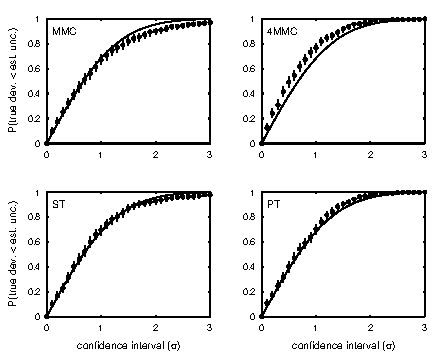
\includegraphics{chapters/wham/figures/confidence-all-1D}}
  \end{center}
  \caption{{\bf Confidence curves for Metropolis Monte Carlo simulations on the 1D model potential.}  The fraction of statistically independent blocks for which the true uncertainty (the deviation of the estimated expectation over the block from the mean of the block estimates) is less than a multiplier of the predicted $1\sigma$ uncertainty (here plotted as the independent variable).  The solid curve shows the fraction expected to fall within the interval for the normal distribution.  Ideally, the curves would coincide.  The results are shown for (MMC) a single Metropolis Monte Carlo simulation at $\beta = 4$; (4MMC) a set of four independent canonical simulations spanning the range $\beta$ = 1 -- 4; (ST) a simulated tempering simulation spanning $\beta$ = 1 -- 4; (PT) a parallel tempering simulation with four replicas spanning $\beta$ = 1 -- 4.  Uncertainties, with 95\% confidence intervals shown here as vertical bars, were computed as described in Appendix \ref{wham:appendix:confidence-uncertainties}.}
  \label{wham:figure:1D-model-confidence-curves}
\end{figure}    

\subsection{Alanine Dipeptide in Implicit and Explicit Solvent.}
\label{wham:section:alanine-dipeptide-simulations}

To illustrate the utility and verify the correctness of the procedures described above for simulations of biological interest, we demonstrate their use in the analysis of parallel tempering simulations of alanine dipeptide in implicit and explicit solvent.  A similar strategy to the 1D model system described above was adopted, with a long simulation partitioned into short blocks (here, 2 ns/replica per block) whose expectations were verified to be statistically independent by the same procedure described above.

Using the {\tt LEaP} program from the AMBER7 molecular mechanics package \cite{AMBER7}, a terminally-blocked alanine peptide (sequence ACE-ALA-NME, see Figure \ref{wham:figure:alanine-dipeptide}) was generated in the extended conformation.  For the explicit solvent system, the peptide was solvated with 431 TIP3P water molecules \cite{jorgensen:1983a} in a truncated octahedral simulation box whose dimensions were chosen to ensure a minimum distance to the box boundaries from the initial extended peptide configuration of $7$\AA.  Peptide force field parameters were taken from the {\tt parm96} parameter set \cite{AMBER-parm96}.  For the implicit solvent simulation, the Generalized Born method of Tsui and Case \cite{tsui:2000a} (corresponding to the flag {\tt igb=1}) was employed with radii from AMBER6, along with a surface area penalty term of the default 5 cal mol$^{-1}$ \AA$^{-2}$.  Covalent bonds to hydrogen were constrained with SHAKE using a tolerance of $10^{-8}$ \AA$ $ \cite{SHAKE}.  Long-range electrostatics for the explicit solvent simulation were treated by the particle-mesh Ewald (PME) method \cite{darden:1993a} with default settings.

\begin{figure}[tb]
  \begin{center}
    \resizebox{2in}{!}{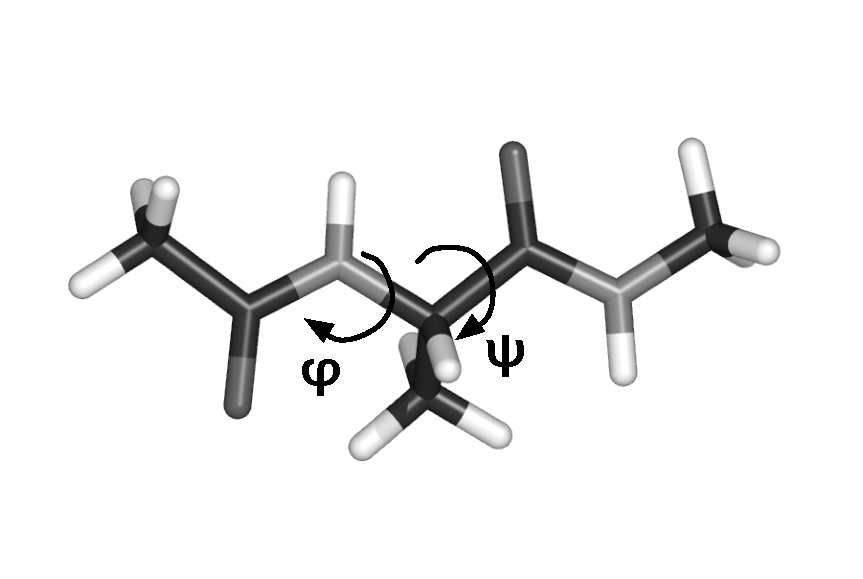
\includegraphics{chapters/wham/figures/alanine-dipeptide}}
  \end{center}
  \caption{{\bf Terminally-blocked alanine peptide with \mbox{\boldmath{$(\phi,\psi)$}} torsions labeled.}}
  \label{wham:figure:alanine-dipeptide}
\end{figure}

Each system was first subjected to 50 steps of steepest descent energy minimization, followed by 1000 steps of conjugate gradient optimization.  To equilibrate the explicit solvent system to the appropriate volume, a 100 ps molecular dynamics simulation was performed with the temperature adjusted to 300 K and the pressure to 1 atm by the Berendsen weak-coupling algorithm \cite{berendsen:1984a} with temperature and pressure relaxation time constants of 1 ps and 0.2 ps, respectively.  The simulation box was fixed at the final size obtained from this equilibration step, with a volume of 13 232 \AA$^3$, in all subsequent simulations.

A parallel tempering (or replica-exchange among temperatures) molecular dynamics simulation \cite{sugita:1999a} was conducted using a parallel {\tt Perl} wrapper for the {\tt sander} program\footnote{A copy of this Perl wrapper to perform replica-exchange simulations using AMBER7 and AMBER8 can be obtained from \url{http://www.dillgroup.ucsf.edu/~jchodera/code/rex}.}.  Replica temperatures were exponentially distributed over the range 273-600K, with 10 replicas required for the implicit solvent simulation (yielding an exchange acceptance probability between neighboring temperatures of approximately $75\%$) and 40 replicas for the explicit solvent simulation (yielding an acceptance probability of approximately $50\%$).  All momenta were reassigned from the Maxwell-Boltzmann distribution at the appropriate replica temperature after each exchange attempt. Between exchanges, constant-energy, constant-volume molecular dynamics was carried out for the explicit solvent simulation, while the implicit solvent simulation utilized Langevin dynamics with a friction coefficient of 95 ps$^{-1}$ to mimic the viscosity of water.  All dynamics utilized a 2 fs timestep.  The algorithm used to select pairs of replicas for temperature exchange attempts starts from the highest-temperature replica and attempts to swap the configuration for the next-lowest temperature replica using a Metropolis-like criteria, and proceeds down the temperatures in this manner.  On the next iteration, swapping attempts start from the lowest temperature and proceed upward, and this alternation in direction is continued in subsequent pairs of iterations.

Starting all replicas from the minimized or volume-equilibrated configuration described above, 100 iterations were conducted with 1 ps between exchange attempts to equilibrate the replicas to their respective temperatures.  This equilibration run was followed by a production run with 20 ps between exchange attempts, giving a total of 100 ns/replica for the implicit solvent production run and 20 ns/replica for the explicit solvent run.  Solute configurations and potential energies were saved from the production run every 1 ps.  Expectations and uncertainties were again estimated using Listing 1 appearing in the Supplementary Material.

Over 2 ns blocks of simulation time (containing 2000 configurations/replica in each block), we computed the probability of the peptide occupying the $\alpha_R$ conformation at 300K, with $\alpha_R$ here defined as $-105 \le \phi < 0$ and $-124 \le \psi < 28$.  This corresponds to configurations that would be classified as right-handed alpha helical.  To validate the uncertainty estimates, confidence curves of the type description in Section \ref{wham:section:1D-model-potential} were computed and are shown in Figure \ref{wham:figure:alanine-dipeptide-confidence-curves}.  Though the confidence intervals are larger because the data contain fewer independent blocks, the uncertainty estimates are still good indicators of the expected deviation from the true expectation.

The potential of mean force (PMF) for the $\psi$ torsion angle at 300K was also computed, and is shown in Figure \ref{wham:figure:alanine-dipeptide-pmf}.  The computed PMF and uncertainty for a representative block is depicted in the top panel, along with the PMF computed using the entire trajectory.  The deviations of the block PMFs from the whole-simulation estimate fall within the 1$\sigma$ uncertainty bars to the expected degree.  In the lower panel, the uncertainties computed from the representative block are compared to the standard deviation of the PMF computed from all blocks, which should be indicative (to within an order of magnitude) of the uncertainty expected from a simulation of the block length.  These too compare favorably.

It is important to note that our neglect of the uncertainty in the dimensionless free energies, $\{f_l\}$, is only reasonable if the correlation time of the observable of interest is much longer than that of the potential energy.  
When this condition is satisfied, the dominant contribution to the uncertainty in the computed expectation of the observable is due to the small number of effectively independent samples of this observable present in the simulation data.  
To demonstrate that this is the case for systems of interest, we have assessed the relative contribution of the neglected uncertainty in the $\{f_l\}$ to the uncertainty of the estimated probability of the $\alpha_R$ conformation of the alanine dipeptide system considered here.
The resulting contribution is 10 times smaller than the uncertainty due to the time correlation treated above for the explicit solvent system and 100 times smaller for the implicit solvent system.
[footnote\{The impact of the uncertainty in the $\{f_l\}$ on the uncertainty in the estimated observable was computed in the following manner: 
We first computed estimates of the $\{f_l\}$ over all uncorrelated 2 ns/replica blocks of simulation data to form a pool of dimensionless free energies that represent the typical uncertainty in a simulation of this length.
Next, for each 2 ns/replica block, we computed the standard deviation in the estimated $\alpha_R$ probability when all $\{f_l\}$ in this pool were substituted into the WHAM equations.
The mean of this standard deviation over all blocks then provides an estimate of the magnitude of the impact of typical uncertainties in the $\{f_l\}$ on the observable of interest.\}]
However, if the observable has a correlation time comparable to that of the potential energy (e.g., if the expectation of the potential energy itself is of interest) then the uncertainty due to imperfect knowledge of the $\{f_l\}$ can be comparable to the uncertainty due to the correlation in the observable.
In these cases where correlation times are comparable, an algorithm that combines our approach with the T-WHAM method of Gallicchio, et al. \cite{gallicchio:2005a}, which explicitly treats the uncertainty in the $\{f_l\}$ when the potential energy samples are uncorrelated, may provide a superior estimate of the uncertainty in the estimate of the observable.
 
We further note that pathological cases may arise where simulations at neighboring temperatures may have poor energy overlap, resulting in large uncertainties in some of the $\{f_l\}$.
Fortunately, these cases are easily detected by examination of the exchange acceptance rates between neighboring temperatures, where they will be conspicuously low, and detectable early in the simulation.  
Such cases are easily remedied by adjusting the temperature spacing or by the addition of more replicas at intermediate temperatures. 

\begin{figure*}[tb]
  \begin{center}
    \resizebox{3.375in}{!}{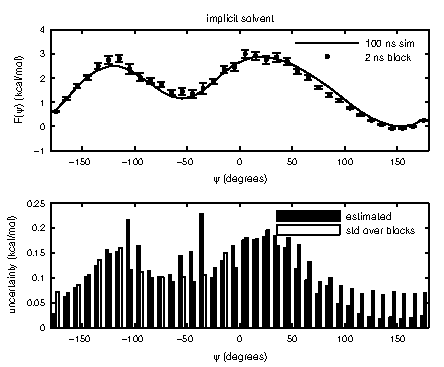
\includegraphics{chapters/wham/figures/pmf-psi-implicit}}
    \resizebox{3.375in}{!}{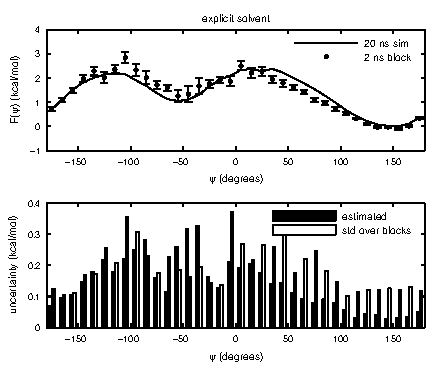
\includegraphics{chapters/wham/figures/pmf-psi-explicit}}
  \end{center}
  \caption{{\bf Potential of mean force in \mbox{\boldmath{$\psi$}} for implicit and explicit solvent parallel tempering simulations.}  Left: implicit solvent; right: explicit solvent. Upper panels: The potential of mean force in the $\psi$ torsion angle at 300 K.  The solid line shows the PMF estimated from the entire simulation, while the filled circles show the estimated PMF uncertainty using the method described in the text for a single 2 ns/replica block.  Lower panels: The computed uncertainties for the same 2 ns block (left bars) along with the average uncertainty expected for a simulation 2 ns/replica in length, estimated from the standard deviation of the PMFs computed from all nonoverlapping blocks of length 2 ns in the full simulation.  All uncertainties are shown as one standard deviation.}
  \label{wham:figure:alanine-dipeptide-pmf}
\end{figure*}

\begin{figure}[tb]
  \begin{center}
    \resizebox{1.65in}{!}{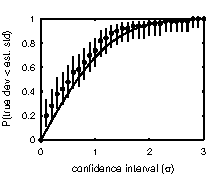
\includegraphics{chapters/wham/figures/confidence-implicit}}
    \resizebox{1.65in}{!}{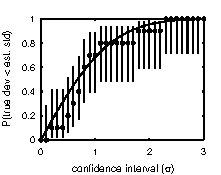
\includegraphics{chapters/wham/figures/confidence-explicit}}
  \end{center}
  \caption{{\bf Confidence curves for implicit and explicit solvent parallel tempering simulations.}  As in Figure \ref{wham:figure:1D-model-confidence-curves}, the fraction of statistically independent 2 ns blocks for which the true uncertainty is less than a multiplier of the predicted $1\sigma$ uncertainty is shown.  The observable used is an indicator function for the $\alpha_\mathrm{R}$ configuration.  Left: implicit solvent (statistics over 50 blocks); right: explicit solvent (statistics over 10 blocks).}
  \label{wham:figure:alanine-dipeptide-confidence-curves}
\end{figure}

%% PRACTICAL CONSIDERATIONS %%%%%%%%%%%%%%%%%%%%%%%%%%%%%%%%%%%%%%%%%%%%%%%%%%%%
\section{Practical Considerations}
\label{wham:section:practical-considerations}

Several issues of great importance to successful implementation of the algorithm have received little discussion in the literature.

\subsection{Choice of Bin Width and Number of Bins.}
\label{wham:section:choice-of-bin-width}

There is a bias-variance tradeoff in the choice of energy histogram width.  As the energy bin width increases, the uncertainty in our histogram estimator for $p_m(\beta)$, the probability density for energy bin $m$, decreases.  At the same time, one expects the resulting estimate of the density of states $\Omega_m$ to become increasingly biased, especially considering the dependence of $p(U)$ on the rapidly-varying exponential Boltzmann factor $e^{-\beta U}$.  Because of this, a reasonable assumption might be that the bin width $\Delta U$ should be chosen such that $\Delta U \ll k_B T$.  However, if the bin size is too small, the uncertainty in the estimate for the $p_m(\beta)$ will be large.  One possibility might be to use a data-based choice of histogram bin width, as in Wand \cite{wand:1997a}, which uses concepts from non-parametric density estimation in attempting to minimize the mean integrated square error (MISE) to the true probability density.

For the alanine dipeptide simulations described in Section \ref{wham:section:alanine-dipeptide-simulations} above, we find that the estimated probability of occupying the $\alpha_\mathrm{R}$ region of conformation space is largely insensitive to the number of bins used to discretize the sampled potential energy range.  In fact, the variation in the computed expectation is well within the statistical uncertainty over the range of 50 to 5000 bins (corresponding to a range of bin widths of 0.5 $k_B T$ to 50 $k_B T$).

\subsection{Computing Integrated Correlation Times.}
\label{wham:section:fast-integrated-correlation-estimates}

Estimating the correlation time $\tau$, defined above in Eqs.\ \ref{wham:equation:integrated-autocorrelation-time-definition} and \ref{wham:equation:autocorrelation-definition}, can be difficult when one is confronted with noisy correlation functions.  While ensuring trajectories are many times longer than the longest correlation times is necessary for an accurate estimate, even if this is achieved, performing the straightforward sum over the entirety of the correlation function $C_t$ as in Eq.\ \ref{wham:equation:integrated-autocorrelation-time-definition} is almost always a poor choice, as the uncertainty in the computed correlation function grows approximately linearly with the lag time $t$ \cite{zwanzig:1969a}.  Even for trajectories many times longer than the correlation length, this sum will be dominated by contributions from the noisy tail, likely resulting in large errors or even negative values for the computed correlation time $\tau$.  Janke proposes a self-consistent approach where the summation is performed only out to lag times of $6 \tau$, after which the correlation function is assumed to be negligible \cite{janke:2002a}.  Evertz contends that this approach produces incorrect results \cite{evertz:2003a}, instead proposing an exponential fit to the tail of the correlation function and use of this fit to evalute the summand when the correlation function is dominated by noise.  Neither solution is both stable and straightforward to apply, so we instead truncate the sum when the normalized fluctuation correlation function $C_t$ first crosses zero, since it is likely unphysical for the correlation function to be negative for most observables\footnote{Velocity correlation functions, where there is often a clear negative peak at short times, are an obvious exception.}.  The zero crossing is an indication that the statistical uncertainty dominates the signal, and that the remainder of the correlation function should be considered indistinguishable from zero.

For most systems and observables, the correlation function will decay rapidly at first and then slowly, approximately exponentially for large $t$.  To avoid the expense of computing $C_t$ at each value of $t$ while still obtaining reasonably accurate integrated correlation times for observables with very different decay timescales, we use an adaptive integration scheme in which the correlation function $C_t$ is computed only at times $t_i = 1 + i(i-1)/2$, where $i = 1,2,3,\ldots$.  In computing the correlation time $\tau$, the sum in Eq.\ \ref{wham:equation:integrated-autocorrelation-time-definition} is now performed only over the $t_i$ terms, with each term weighted by $t_{i+1} - t_i$, with $t_1 = 1$.  This approach ensures high time resolution at small $t$ when $C_t$ is likely to be rapidly changing but avoids the expense of computing $C_t$ at every $t$ in the slowly-decaying tails.  We find the accuracy of this approach to be acceptable --- differences typically amount to at most ten percent.

\subsection{Neglect of Bin Statistical Inefficiencies $g_{kn}$.}
\label{wham:section:neglect-of-bin-statistical-inefficiencies}

It is often assumed or stated without justification that the energy bin statistical inefficiencies $g_{mk}$ appearing in Eqs.\ \ref{wham:equation:optimal-dos} and \ref{wham:equation:parallel-tempering-dos}, representing the number of snapshots required for a statistically independent sampling of the energy bin, are all equal or equal to unity \cite{kumar:1992a,sugita:1999a,okamoto:2004a}.  All $g_{mk}$ will be equal to unity only if the $\{\psi_{mkn}\}_{n = 1}^{N_k}$ are uncorrelated.  To test this assumption, we have computed the statistical inefficiencies for the systems mentioned in Section \ref{wham:section:applications} above.  To our knowledge, this is the first time a test of this claim has been reported in the literature.  Indeed, for the explicit solvent system studied in Section \ref{wham:section:alanine-dipeptide-simulations} above, we find large differences in the statistical inefficiencies for the same replica but different energy bins, sometimes differing up to two orders of magnitude.  Similarly, for the same energy bin, the statistical inefficiencies from different replicas can differ by up to two orders of magnitude.

In the limit that our parallel tempering simulation is very long --- long enough for each replica to execute an unrestricted random walk through all temperatures and explore all relevant regions of configuration space --- each replica can be considered to be equivalent. In this case, the statistical inefficiencies should be independent of replica index $k$, and we can write $g_m$ as the statistical inefficiency for energy bin $m$.  Applied to Eqs.\ \ref{wham:equation:parallel-tempering-dos} and \ref{wham:equation:parallel-tempering-dos-uncertainty}, this yields a new set of expressions:
\begin{eqnarray}
\estimator{\Omega}_m &=& \frac{\sum\limits_{k=1}^K H_{mk}}{\sum\limits_{k=1}^{K} \sum\limits_{l=1}^{L} N_{kl} \, \Delta U \, \exp[f_{l} - \beta_{l} U_m]} \\
\delta^2 \estimator{\Omega}_m &=& \frac{\estimator{\Omega}_m}{g_m^{-1}  \sum\limits_{k = 1}^{K} \sum\limits_{l=1}^{L} N_{kl} \, \Delta U \, \exp[f_l - \beta_l U_m]}
\end{eqnarray}
The quantity $\sum_{k=1}^K N_{kl}$, simply represents the total number of configurations stored from any replica at temperature $\beta_l$.  For a parallel tempering simulation, where each temperature must be populated by exactly one replica at all times, this is simply $N$, the total number of configurations stored per replica.  Additionally, $H_m \equiv \sum_{k=1}^K H_{mk}$ is the total number of configurations over all replicas (and hence temperatures) with energy in bin $m$.  This gives
\begin{eqnarray}
\estimator{\Omega}_m &=& \frac{H_m}{N \sum\limits_{l=1}^L \exp[f_l - \beta_l U_m]}
\end{eqnarray}
which is identical to the WHAM result for independent canonical simulations for the case where all $g_{mk}$ are identical or unity.  If there is no correlation in the data --- that is, all configurations are independent --- it does not matter whether we apply this analysis to the original data or collect up the configurations by temperature and apply WHAM equations for independent canonical simulations.  This expression is in fact identical to the one used in many published works that have previously attempted to use the weighted histogram analysis method for the analysis of parallel tempering simulations, such as \cite{sugita:1999a,okamoto:2004a}.

Under these same assumptions, the correlation functions for any observable $A$ should also be identical for each replica.  One can therefore average estimates of the unnormalized correlation functions $\expect{A_n A_{n+t}}$ over the replicas and use optimal estimates of the mean and variance computed over all of the replicas to obtain an optimal estimate of the statistical inefficiencies and uncertainties.  An implementation illustrating this procedure is provided in the Supplementary Material as Listing 2. 

Note, however, that the above assumptions of equivalence cannot be made in cases where the replicas are clearly \emph{inequivalent}, such as in a simulated tempering replica-exchange (STREM) simulation \cite{mitsutake:2000a,mitsutake:2004a}.  In that case, the expression above will only be recovered if the time between samples is so long that all the $g_{mk}$ are unity.

\subsection{The Statistical Inefficiency for the Cross-Correlation Term, $g_{k,wA;w}$.}

In computing the statistical inefficiency for the cross-correlation term, uncertainties in the computed integrated autocorrelation times due to insufficient data or approximations may cause the cross-correlation term to dominate and the estimate of the square uncertainty of $\estimator{A}$ (eq \ref{wham:equation:uncertainty-in-canonical-A}) to be negative.  Clearly, this should not be allowed to occur, as the squared-uncertainty should be a strictly positive quantity.

The statistical inefficiencies $g$ should obey the following relation (derived in Appendix \ref{wham:appendix:statistical-inefficiency-relation}):
\begin{eqnarray}
g_{x;y} &\le& ( g_x \, g_y )^{1/2} \, \frac{\sigma_x \sigma_y}{|\sigma^2_{x;y}|} \label{wham:equation:statistical-inefficiency-relation}
\end{eqnarray}
This is often violated when the correlation function is noisy, and can lead to negative estimates of the squared uncertainty when the cross-correlation term dominates.  In these cases, we find it best to simply limit $g_{x;y}$ to its maximum allowed value computed from the right-hand side of Eq.\ \ref{wham:equation:statistical-inefficiency-relation}.  Since the autocorrelation times are usually shorter than the cross-correlation time, it is believed that these estimates will be better than the integrated cross-correlation time.

%\subsection{Unbiased estimator for correlation time.}
%
%Flyvbjerg points out that our estimator for the uncertainty in an expectation, $\delta^2 \hat A$, is biased, and proposed the unbiased estimator \cite{flyvbjerg:1989a}
%\begin{eqnarray}
%\delta^2 \hat A &=& \frac{\sigma^2 \, (1 + 2 \tau)}{N - (2 N_c+1) + N_c (N_c+1) / N} 
%\end{eqnarray}
%where $N_c$ is point at which the sum was truncated in the computation of $\tau$.
%
% In practice, this is not entirely useful, since the assumption that $N_c << N$ is often violated.
%
%\subsection{Second-order corrections to the estimator and uncertainty.}
%
%In some cases, the first-order Taylor expansion of Eqn. \ref{wham:equation:uncertainty-in-canonical-A} may not be sufficient, and the contribution to the bias and uncertainty from higher-order terms may be significant.  Luckily, much of the second-order expansion can be incorporated without requiring additional uncertainties to be computed.  Higher-order versions of the above equations can be found in Winzer \cite{winzer:2000a}.

%% CONCLUSIONS %%%%%%%%%%%%%%%%%%%%%%%%%%%%%%%%%%%%%%%%%%%%%%%%%%%%%%%%%%%%%%%%%%%%

\section{Conclusion}

We have presented an extension of the weighted histogram analysis method (WHAM) for the analysis of one or more independent simulated tempering or parallel tempering simulations.  The method provides not only estimators of canonical expectations but also estimators for the statistical uncertainties in the resulting estimates.  We hope that, with the availability of the provided example code, workers using these simulation techniques will provide uncertainty estimates so that the statistical significance of results obtained from them can be assessed.  We have shown that the estimator for the expectation has small bias and produces excellent uncertainty estimates for both a 1D model system and a solvated biomolecular system in implcit and explicit solvent.

While other workers had attempted to apply WHAM to simulated or parallel tempering data in the past \cite{mitsutake:2000a,sugita:1999a}, the key advance here is the consideration of the correlated nature of the configurations sampled by each replica as it performs a pseudorandom walk in temperature, allowing a proper assessment of the true number of independent samples present in the data.  This produces correct optimal estimators and makes possible the estimation of statistical uncertainties.  This method can be extended to the analysis of other generalized-ensemble simulations, such as the multicanonical method (MUCA) \cite{berg:1991a,berg:1992a,hansmann:1993a,nakajima:1997a,yasar:2000a}, by consideration of replica correlation times as the system samples various energy levels biased by the estimate of the density of states.  Still, it is important to point out that, while we consider the contribution from time-correlation of the observable to the uncertainty estimate, we currently neglect the contribution of the uncertainty in the per-configuration weights (which originates from the uncertainty in the density of states) to the estimate of the expectation --- we assume it is negligible and await a more complete treatment of the uncertainty in cases where it is not.  

%% ACKNOWLEDGMENTS %%%%%%%%%%%%%%%%%%%%%%%%%%%%%%%%%%%%%%%%%%%%%%%%%%%%%%%%%%%%%%%%%%%%

\section{Acknowledgments}

JDC was supported by an Howard Hughes Medical Institute and an IBM predoctoral fellowship.  WS acknowledges support from NSF MRSEC Center on Polymer Interfaces and Macromolecular Assemblies DMR -- 0213618, and KD the support of NIH grant GM34993.  The authors would like to thank Libusha Kelly, Bosco K. Ho, and M. Scott Shell (University of California, San Francisco) for critical reading of this manuscript, as well as the anonymous referee who raised an excellent point regarding our neglect of the uncertainty in the dimensionless free energies.  This manuscript was strengthened as a result of their input.


%% APPENDIX %%%%%%%%%%%%%%%%%%%%%%%%%%%%%%%%%%%%%%%%%%%%%%%%%%%%%%%%%%%%%%%%%%%%

\section{Relation for Statistical Inefficiencies}
\label{wham:appendix:statistical-inefficiency-relation}

Consider a random process where we make a series of $N$ time-correlated measurements of two (possibly correlated) observables $X$ and $Y$, resulting in the time series $\{x_n,y_n\}_{n=1}^N$. We estimate the quantity $Z = \expect{X}/\expect{Y}$ from our sample means, and wish to compute the uncertainty in our estimate, defined as
\begin{eqnarray}
\delta^2 Z &\equiv& \sigma^2_Z = \expect{(Z-\expect{Z})^2} = \expect{Z^2} - \expect{Z}^2 .
\end{eqnarray}
To first order about $\expect{X}/\expect{Y}$, this uncertainty is given by
\begin{eqnarray}
\sigma^2_Z &=& \left[\frac{\expect{X}}{\expect{Y}}\right]^2 \, \left[ \frac{\sigma^2_X}{\expect{X}^2} + \frac{\sigma^2_Y}{\expect{Y}^2} - 2 \frac{\sigma^2_{X;Y}}{\expect{X} \expect{Y}} \right]
\end{eqnarray}
where $\sigma^2_{X;Y}$ denotes the (not necessarily positive) covariance of the expectations of $X$ and $Y$.  The Schwartz inequality requires that this covariance obey the relation
\begin{eqnarray}
|\sigma^2_{X;Y}| &\le& \sigma_X \sigma_Y
\end{eqnarray}
(see, for example, \cite{casella:statistical-inference}). Given this, we note
\begin{eqnarray}
\left| \frac{\sigma^2_{X;Y}}{\sigma_X \sigma_Y} \right| &\le& 1 \label{wham:equation:variance-bounds}
\end{eqnarray}
Correlation analysis gives estimators for these quantities as
\begin{eqnarray}
\sigma^2_X &=& \sigma^2_x / (g_x^{-1} N) \nonumber \\
\sigma^2_Y &=& \sigma^2_y / (g_y^{-1} N) \nonumber \\
\sigma^2_{X;Y} &=& \sigma^2_{x;y} / (g_{x;y}^{-1} N) \label{wham:equation:variance-definitions}
\end{eqnarray}
where $\sigma^2_x$ denotes the sample variance of the observations $\{x_n\}_{n=1}^N$ and $g$ denotes the statistical inefficiency obtained from the autocorrelation time, \emph{i.e.}
\begin{eqnarray}
g_x = 1 + 2 \tau_x \ge 1.
\end{eqnarray}
Combining Eqs.\ \ref{wham:equation:variance-bounds} and \ref{wham:equation:variance-definitions} gives
\begin{eqnarray}
\frac{| \sigma^2_{x;y}|}{\sigma_x \, \sigma_y} \cdot \frac{g_{x;y}}{( g_x \, g_y )^{1/2}} &\le& 1
\end{eqnarray}
where we have moved the statistical inefficiencies and variances out of the absolute value, as they are always positive.  Finally, we obtain an upper bound for $g_{x;y}$:
\begin{eqnarray}
g_{x;y} &\le& ( g_x \, g_y )^{1/2} \, \frac{\sigma_x \sigma_y}{|\sigma^2_{x;y}|}
\end{eqnarray}
In using numerical methods to estimate the statistical inefficiencies $g$ from finite trajectories, this inequality may not hold, sometimes leading to negative squared uncertainties.  Limiting the estimated $g_{x;y}$ by capping it at this value will prevent this from occurring.

\section{Uncertainty Estimates for Confidence Curves}
\label{wham:appendix:confidence-uncertainties}

To estimate the uncertainties in Figures \ref{wham:figure:1D-model-confidence-curves} and \ref{wham:figure:alanine-dipeptide-confidence-curves}, a Bayesian inference scheme was used.  Since the expectations computed from each block are independent, the number of blocks $n$ that fall inside the given scaled deviation $\sigma$ is described by a binomial distribution with parameter $\theta$, true (unknown) probability that the blocks fall within the given deviation $\sigma$:
\begin{eqnarray}
P(n | \theta) &=& \frac{N!}{n! (N-n)!} \theta^n (1-\theta)^{N-n}
\end{eqnarray}
We can write the posterior distribution for the probability $p$ given the observed number of blocks within the given deviation $n$ using Bayes' rule
\begin{eqnarray}
p(\theta | n) &\propto& p(n | \theta) \, p(\theta)
\end{eqnarray}
where $p(\theta)$ is the prior distribution for the parameter $\theta$.  If we choose the prior $p(\theta)$ to be a Beta distribution with hyperparameters $\alpha$ and $\beta$, given by
\begin{eqnarray}
p(\theta | \alpha, \beta) &=& [B(\alpha, \beta)]^{-1} x^{\alpha - 1} (1-x)^{\beta-1}
\end{eqnarray}
where $B(\alpha, \beta)$ is the beta function, then the posterior $p(\theta | n)$ will also be a Beta distribution with parameters $n + \alpha$ and $(N-n) + \beta$, as the Beta distribution is a conjugate prior to the Binomial distribution.  We take the hyperparameters $\alpha$ and $\beta$ to be unity to make the prior distribution uniform, resulting in a posterior $\theta \sim \mathrm{Beta}(n+1, N-n+1)$.  A 95\% central confidence interval, corresponding to the location where the cumulative distribution function for the Beta distribution reaches the values of 0.025 and 0.0975, was plotted.

%
%%% END DOCUMENT
%\end{document}
